% The comment below tells Rubber to compile the .dot files.
%
% rubber: module graphics
% rubber: rules rules.ini

\documentclass{beamer}

\usetheme{default}

\usefonttheme{structurebold}
\usepackage{helvet}
\usecolortheme{seagull}         % white on black

\usepackage[utf8]{inputenc}
\PassOptionsToPackage{hyphens}{url}\usepackage{hyperref,xspace,multicol}
\usepackage[absolute,overlay]{textpos}
\usepackage{tikz}
\usetikzlibrary{arrows,shapes,trees,shadows,positioning}
\usepackage{fancyvrb}           % for \Verb

% Remember the position of every picture.
\tikzstyle{every picture}+=[remember picture]

\tikzset{onslide/.code args={<#1>#2}{%
  \only<#1>{\pgfkeysalso{#2}} % \pgfkeysalso doesn't change the path
}}

% Colors.
\definecolor{guixred1}{RGB}{226,0,38}  % red P
\definecolor{guixorange1}{RGB}{243,154,38}  % guixorange P
\definecolor{guixyellow}{RGB}{254,205,27}  % guixyellow P
\definecolor{guixred2}{RGB}{230,68,57}  % red S
\definecolor{guixred3}{RGB}{115,34,27}  % dark red
\definecolor{guixorange2}{RGB}{236,117,40}  % guixorange S
\definecolor{guixtaupe}{RGB}{134,113,127} % guixtaupe S
\definecolor{guixgrey}{RGB}{91,94,111} % guixgrey S
\definecolor{guixdarkgrey}{RGB}{46,47,55} % guixdarkgrey S
\definecolor{guixblue1}{RGB}{38,109,131} % guixblue S
\definecolor{guixblue2}{RGB}{10,50,80} % guixblue S
\definecolor{guixgreen1}{RGB}{133,146,66} % guixgreen S
\definecolor{guixgreen2}{RGB}{157,193,7} % guixgreen S

\setbeamerfont{title}{size=\huge}
\setbeamerfont{frametitle}{size=\huge}
\setbeamerfont{normal text}{size=\Large}

% White-on-black color theme.
\setbeamercolor{structure}{fg=guixorange1,bg=black}
\setbeamercolor{title}{fg=white,bg=black}
\setbeamercolor{date}{fg=guixorange1,bg=black}
\setbeamercolor{frametitle}{fg=white,bg=black}
\setbeamercolor{titlelike}{fg=white,bg=black}
\setbeamercolor{normal text}{fg=white,bg=black}
\setbeamercolor{alerted text}{fg=guixyellow,bg=black}
\setbeamercolor{section in toc}{fg=white,bg=black}
\setbeamercolor{section in toc shaded}{fg=white,bg=black}
\setbeamercolor{subsection in toc}{fg=guixorange1,bg=black}
\setbeamercolor{subsection in toc shaded}{fg=white,bg=black}
\setbeamercolor{subsubsection in toc}{fg=guixorange1,bg=black}
\setbeamercolor{subsubsection in toc shaded}{fg=white,bg=black}
\setbeamercolor{frametitle in toc}{fg=white,bg=black}
\setbeamercolor{local structure}{fg=guixorange1,bg=black}

\newcommand{\highlight}[1]{\alert{\textbf{#1}}}

\title{GNU~Guix is 4 years old!}

\author{Ludovic Courtès}
\date{\small{GNU Hackers Meeting, Rennes, August 2016}}

\setbeamertemplate{navigation symbols}{} % remove the navigation bar

\AtBeginSection[]{
  \begin{frame}
    \frametitle{}
    \tableofcontents[currentsection]
  \end{frame} 
}


\newcommand{\screenshot}[1]{
  \begin{frame}[plain]
    \begin{tikzpicture}[remember picture, overlay]
      \node [at=(current page.center), inner sep=0pt]
        {\includegraphics[width=\paperwidth]{#1}};
    \end{tikzpicture}
  \end{frame}
}


\begin{document}

\maketitle

\setbeamercolor{normal text}{bg=guixblue2}
\begin{frame}
  \Huge{\textbf{The rise and fall of distros.}}
\end{frame}
\setbeamercolor{normal text}{fg=white,bg=black}

%% \begin{frame}[plain]
%%   \Huge{It's worse, really.}
%% \end{frame}

%% \setbeamercolor*{normal text}{bg=guixdarkgrey,fg=white}
%% \begin{frame}[plain]
%%   \Large{``Let's Package jQuery: A Javascript Packaging Dystopian
%%     Novella'' by Chris Webber}
%%   \\[2.cm]
  
%%   \url{http://dustycloud.org/blog/javascript-packaging-dystopia/}
%% \end{frame}
%% \setbeamercolor*{normal text}{fg=white,bg=black}

\setbeamercolor{normal text}{bg=guixred3,fg=white}
\begin{frame}[plain]
  \begin{quotation}
    \noindent
    \LARGE{``Debian and other distributions are going to be \textbf{that
        thing you run docker on}, little more.''}
  \end{quotation}
  \hfill{--- Jos Poortvliet, ownCloud developer}

  \begin{tikzpicture}[overlay]
    \node [at=(current page.south east), anchor=south east]{
      \url{http://lwn.net/Articles/670566/}
    };
  \end{tikzpicture}
\end{frame}
\setbeamercolor{normal text}{fg=white,bg=black}

\begin{frame}[plain]
  \begin{tikzpicture}[remember picture, overlay]
    \node [at=(current page.center), inner sep=0pt]
          {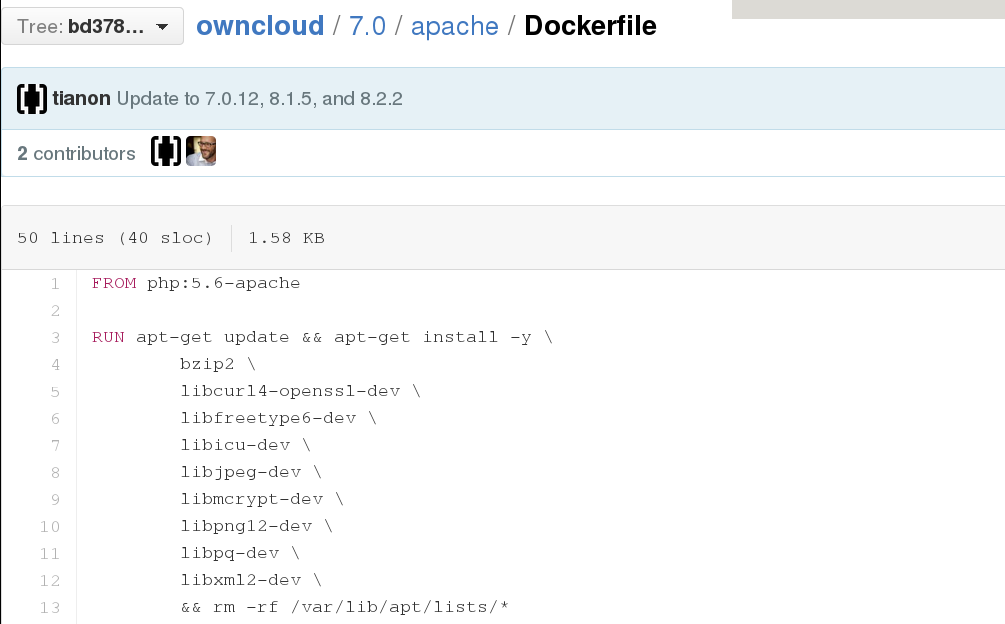
\includegraphics[width=\paperwidth]{images/dockerfile-owncloud-cropped}};

    \node [at=(current page.center), anchor=south west, overlay,
           text=black, text opacity=1, fill=white, opacity=.7, text width=5cm]
          {\LARGE{It's also that thing you run \emph{inside} Docker!}};
  \end{tikzpicture}
\end{frame}

\begin{frame}[plain]
  \LARGE{
    main griefs:
  \begin{itemize}
  \item distros are \textbf{inflexible}
  \item distros \textbf{``lag behind''}
  \item developers have to \textbf{``chase distros''}
  \end{itemize}
  }
\end{frame}

\setbeamercolor{normal text}{bg=white}
\screenshot{images/package-managers-cropped}
\screenshot{images/npm-curl-pipe-sh-cropped}

\begin{frame}[plain]
  \begin{tikzpicture}[remember picture, overlay]
    \node [at=(current page.center), inner sep=0pt]
          {\includegraphics[height=\paperheight]{images/universal_install_script}};
    \node [at=(current page.north east), anchor=south east, rotate=90,
           text=black, text opacity=1, fill=white, opacity=.6]{
      \url{http://xkcd.com/1654/}
    };
  \end{tikzpicture}
\end{frame}

\setbeamercolor{normal text}{bg=black}

\begin{frame}[plain]
  \Huge{\textbf{Giving up?}}
  \\[1.0cm]
  \uncover<2->{\Large{$\rightarrow$ ``app bundles''}}
\end{frame}

\screenshot{images/dockerfile-owncloud-cropped}

\begin{frame}[plain]
  \begin{tikzpicture}[remember picture, overlay]
    \node [at=(current page.center), inner sep=0pt]
          {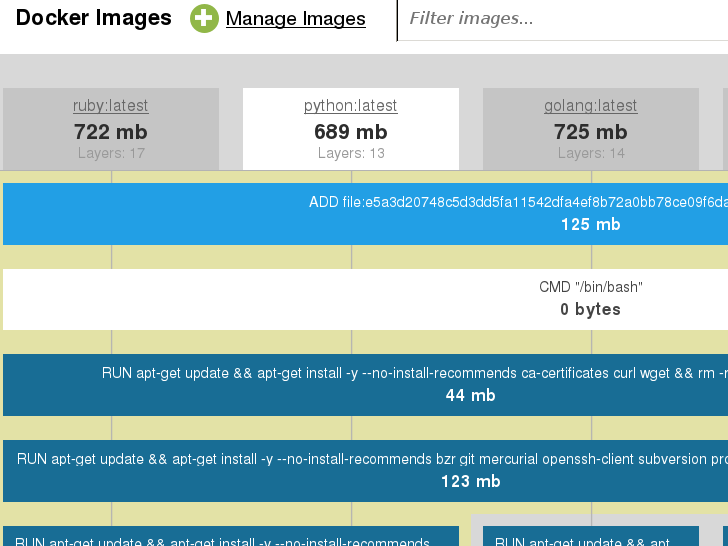
\includegraphics[width=\paperwidth]{images/docker-image-layers-cropped}};
    \node [at=(current page.north east), anchor=north east,
           text=black, text opacity=1, fill=white, opacity=.6]{
      \url{https://imagelayers.io/}
    };
  \end{tikzpicture}
\end{frame}

\setbeamercolor{normal text}{bg=guixdarkgrey,fg=white}
\begin{frame}[plain]
  \Huge{... still too low-level}
  \\[1cm]
  \uncover<2->{\Huge{Maybe what we need is an \textbf{app store} that
      \emph{feels} like apt, yum \& co.?}}
\end{frame}
\setbeamercolor{normal text}{bg=black,fg=white}

\screenshot{images/arstechnica-snappy-goodbye-apt-yum}

\setbeamercolor{normal text}{bg=guixred3,fg=white}
\begin{frame}[plain]
  \begin{quotation}
    \noindent
    \LARGE{``This is, to put it diplomatically, a heaping pile of
      steaming bullshit [...] served by the Canonical press
      department.''}
    \\[6mm]
    \LARGE{\uncover<2->{``There is in fact another system with very
        similar goals, which is now called \textbf{Flatpak} [...]''}}
  \end{quotation}
  \hfill{--- Adam Williamson (Red Hat, Fedora)}

  % https://www.happyassassin.net/2016/06/16/on-snappy-and-flatpak-business-as-usual-in-the-canonical-propaganda-department/
  \begin{tikzpicture}[overlay]
    \node [at=(current page.south east), anchor=south east]{
      \url{https://www.happyassassin.net/}
    };
  \end{tikzpicture}
\end{frame}
\setbeamercolor{normal text}{fg=white,bg=black}


\screenshot{images/flatpak}

\begin{frame}[plain]
  \begin{tikzpicture}[remember picture, overlay]
    \node [at=(current page.center), inner sep=0pt]
          {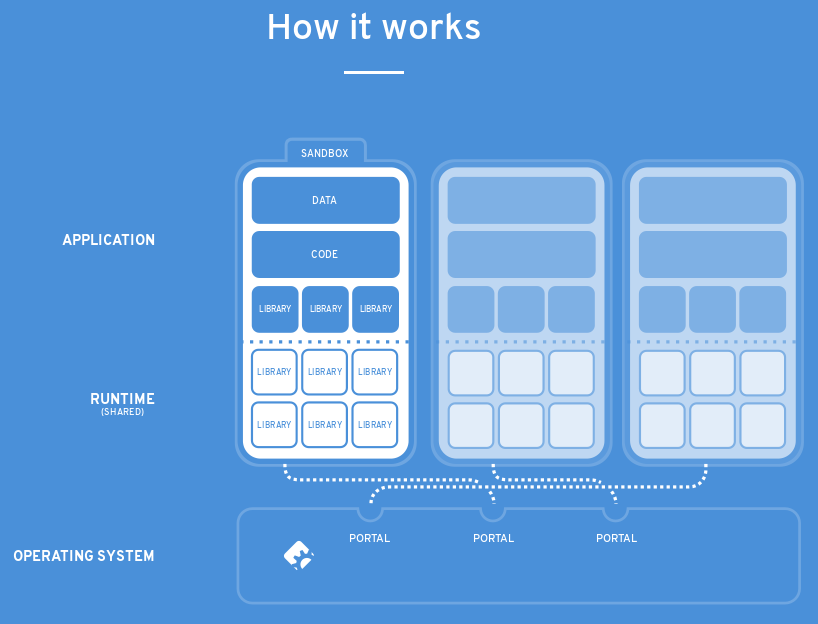
\includegraphics[width=\paperwidth]{images/flatpak-how-it-works-cropped}};
    \node [at=(current page.north east), anchor=north east,
           text=black, text opacity=1, fill=white, opacity=.6]{
      \url{http://flatpak.org/}
    };
  \end{tikzpicture}
\end{frame}


\begin{frame}[plain]{``app bundles'' are headed wrong}
  \Large{
    \begin{itemize}
    \item difficulty to \highlight{compose} software packages
    \item no ``big picture'' \highlight{integration work}
    \item where's the \highlight{Corresponding Source}?
    \item \textbf{``app'' model/free software commons mismatch}
    \end{itemize}
  }
\end{frame}

%% \screenshot{images/frozen-pizza}
%% \screenshot{images/docker-security}

% TODO: http://www.vitavonni.de/blog/201503/2015031201-the-sad-state-of-sysadmin-in-the-age-of-containers.html

%%%%%%%%%%%%%%%%%%%%%%%%%%%%%%%%%%%%%%%%%%%%%%%%%%%%%%%%%%%%%%%%%%%%%%%%%%%%%%
\setbeamercolor{normal text}{fg=black,bg=white}
\screenshot{images/GuixSD-horizontal-print}
\setbeamercolor{normal text}{fg=white,bg=black}

\begin{frame}{Guix}
  \LARGE{
    \begin{enumerate}
    \item transactional package manager
    \item software environment manager
    \item APIs \& tools to customize environments
    \item packaging tools
    \end{enumerate}
  }
\end{frame}

\begin{frame}[fragile]

  \begin{semiverbatim}
\$ guix package -i gcc-toolchain coreutils sed grep
\textrm{...}

\$ eval `guix package --search-paths`
\textrm{...}

\$ guix package --manifest=my-software.scm
\textrm{...}
  \end{semiverbatim}

  %% \begin{tikzpicture}[overlay]
  %%   \node[rounded corners=4, text centered,
  %%         fill=guixorange1, text width=3cm,
  %%         inner sep=3mm, rotate=5, opacity=.75, text opacity=1,
  %%         drop shadow={opacity=0.5}] at (5, 4) {
  %%           \textbf{\large{demo}}
  %%         };
  %% \end{tikzpicture}
\end{frame}

\setbeamercolor{normal text}{bg=guixdarkgrey,fg=guixred3}
\begin{frame}[fragile]
  \Huge{Want to get started hacking on GIMP?}
  \\[2cm]
  \uncover<2->{\Large{A simple matter of installing the deps, right?}}
\end{frame}

\setbeamercolor{normal text}{bg=white}
\begin{frame}[plain]
  \begin{tikzpicture}[remember picture, overlay]
    \node [at=(current page.center), inner sep=0pt]
          {\includegraphics[width=\paperwidth]{images/gimp-graph}};
  \end{tikzpicture}
\end{frame}
\setbeamercolor{normal text}{fg=white,bg=black}


\begin{frame}[fragile]
  \begin{semiverbatim}
\$ guix environment --container gimp
\textrm{...}

\$ guix environment --container gimp \\
     --ad-hoc git autoconf automake gdb
\textrm{...}

  \end{semiverbatim}
\end{frame}

\begin{frame}[plain]
  \Huge{Creating package variants at the command line}
\end{frame}

\begin{frame}[fragile]
  \begin{semiverbatim}
\$ guix package -i emacs \\
    \alert<1>{--with-source}=./emacs-25.1rc0.tar.gz
\textrm{...}

\pause
\$ guix package -i git \\
     \alert<2>{--with-input}=openssl=libressl
\textrm{...}

  \end{semiverbatim}
\end{frame}

\begin{frame}[plain]
  \Huge{Your personal packages or variants in
    \texttt{GUIX\_PACKAGE\_PATH}!}
\end{frame}

\begin{frame}[plain]
  \Huge{Security updates ``grafted'' onto available binaries}
\end{frame}

\screenshot{images/gimp-graph}

\begin{frame}[plain]
  \begin{tikzpicture}[remember picture, overlay]
    \node [at=(current page.center), inner sep=0pt]
          {\includegraphics[width=\paperwidth]{images/os-declaration}};
    \node [at=(current page.center), fill=black, opacity=.3, text
      opacity=1., minimum height=21cm, minimum width=297mm]
          {\huge{\textbf{GuixSD: declarative OS config}}};
  \end{tikzpicture}
\end{frame}

\begin{frame}[fragile]
  \begin{overlayarea}{\textwidth}{8cm}
  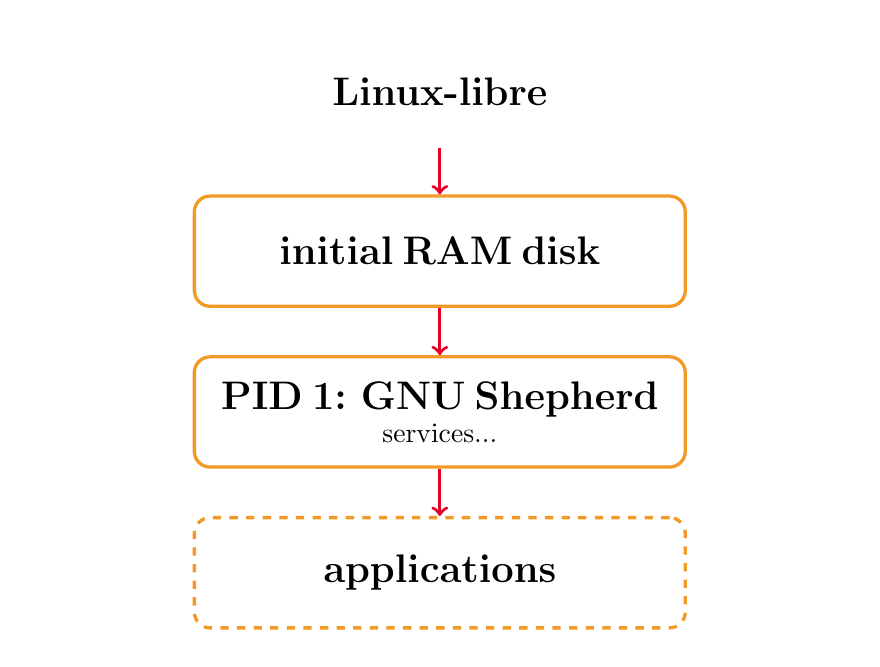
\begin{tikzpicture}[kernel/.style = {
                        text width=10cm, minimum height=1.4cm,
                        text centered,
                        rounded corners=2mm,
                        fill=white, text=black
                      },
                      userland/.style = {
                        draw=guixorange1, very thick,
                        fill=white, text=black, text width=6cm,
                        rounded corners=2mm, minimum height=1.4cm,
                        text centered
                      }]
    \matrix[row sep=6mm, column sep=1cm] {
      \node(kernel)[kernel]{\textbf{\Large{Linux-libre}}};
      \\

      \node<2->(initrd)[userland]{\textbf{\Large{initial RAM disk}}};
      \\

      \node<4->(shepherd)[userland]{\textbf{\Large{PID 1: GNU Shepherd}}
        \\ services...};
      \\

      \node<6->(user)[userland, dashed]{\textbf{\Large{applications}}};
      \\
    };

    \path[->, very thick, draw=guixred1]<2->
      (kernel) edge (initrd);
    \path[->, very thick, draw=guixred1]<4->
      (initrd) edge (shepherd);
    \path[->, very thick, draw=guixred1]<6->
      (shepherd) edge (user);
    
  \end{tikzpicture}
  \end{overlayarea}

  \begin{tikzpicture}[overlay,
                      guile/.style = {
                         fill=guixyellow, text=black, rotate=30,
                         rounded corners=4mm, text width=3cm,
                         opacity=.75, text opacity=1, text centered,
                         minimum height=1.3cm
                      }]
    \node<3->(labelinitrd) [guile] at (initrd.east) {%
      \Large{Guile}
    };
    \node<5->(labelinitrd) [guile] at (shepherd.east) {%
      \Large{Guile}
    };
  \end{tikzpicture}
\end{frame}

\setbeamercolor{normal text}{bg=guixblue2}
\begin{frame}[plain]
  \Huge{\textbf{Status.}}
\end{frame}
\setbeamercolor{normal text}{fg=white,bg=black}

\begin{frame}{4 years!}
  \begin{itemize}
    \item Aug. 2012 --- GNU Hackers Meeting, Düsseldorf
    \item Nov. 2012 --- dubbed GNU
    \item{Jan. 2013 --- \alert{0.1}}
    \item ...
    \item{July 2014 --- \alert{0.7}, \textbf{installable operating
        system}}
    \item ...
    \item{Nov. 2015 --- \alert{0.9.0}, new service framework, etc.}
    \item{Jan. 2016 --- successful \alert{fundraiser} for new
      \textbf{build farm}}
    \item{Mar. 2016 --- \alert{0.10.0}, grafts, GNOME}
    \item{Aug. 2016 --- \alert{0.11.0}, system tests, more services}
  \end{itemize}
\end{frame}

\screenshot{images/better}

\begin{frame}{growth!}
  \Large{
  \begin{itemize}
    \item 3,800+ packages
    \item 4 architectures
    \item binaries at \url{https://hydra.gnu.org}
    \item $\approx$500 new packages per release
    \end{itemize}
  }
\end{frame}


\setbeamercolor{normal text}{bg=white}
\screenshot{images/openhub-activity}
\screenshot{images/openhub-contributors}
\setbeamercolor{normal text}{bg=black}

\setbeamercolor{normal text}{bg=guixblue2}
\begin{frame}[plain]
  \Huge{\textbf{Scaling up.}}
\end{frame}
\setbeamercolor{normal text}{fg=white,bg=black}

\begin{frame}[fragile]{importers \& updaters}
  \Large{
  \begin{itemize}
  \item{\texttt{guix import}
    \begin{itemize}
    \item \highlight{8.5 importers}: GNU, Nix, PyPI, CPAN, CRAN,
      Hackage, ELPA, Gem, npm (GSoC~2016)
    \end{itemize}}
  \item{\texttt{guix refresh}
    \begin{itemize}
      \item \highlight{11 updaters}: GNU, GNOME, KDE, Xorg, ELPA, CRAN,
        Bioconductor, Hackage, PyPI, Gem, GitHub
    \end{itemize}}
  \item \texttt{guix lint -c cve} (vulnerabilities)
  \end{itemize}
  }
\end{frame}

\begin{frame}{contributions}
  \Large{
  \begin{itemize}
  \item \highlight{documented processes}, code of conduct
  \item \highlight{consensus-based} decision making
  \item \highlight{tools}: \texttt{guix lint} (12 checkers!),
    \texttt{guix build --rounds=2}, etc.
  \item good \highlight{reviews \& mentoring}
  \item<2-> 30 committers, but \highlight{5--10 frequent reviewers}
  \item<3->{50+ emails per day, \highlight{hard to track patches}
    \begin{itemize}
    \item Patchwork? QEMU's \texttt{patches}? suggestions?
    \end{itemize}}
  \end{itemize}
  }
\end{frame}

\begin{frame}{maintainership, responsibilities}
  \Large{
  \begin{itemize}
    \item \highlight{Ricardo Wurmus} co-maintainer since July!
    \item{currently \highlight{$\approx$3 build farm sysadmins}
      \begin{itemize}
      \item ... but heading towards distributed sysadmin!
      \item run GuixSD everywhere, version-control that
      \item eventually: \texttt{guix deploy}
      \end{itemize}}
  \end{itemize}
  }
\end{frame}

\begin{frame}{build farm \& funding}
  \Large{
  \begin{itemize}
    \item \highlight{hardware donated} by FSF, TUM, GNU~Spain,
      individuals
    \item 2 \highlight{Novena} boards (ARMv7) donated by Bunnie
    \item \highlight{raised \$8,000+} in January 2016
    \item \highlight{5,000~EUR donated by Igalia}
    \item ``\highlight{Guix Europe}'' NPO created in France in 2016
  \end{itemize}
  }

  \begin{tikzpicture}[overlay]
    \node<2>[rounded corners=4, text centered,
          fill=guixorange1, text width=5cm,
          inner sep=5mm, opacity=.75, text opacity=1,
          drop shadow={opacity=0.5}] at (5, 3) {
            \textbf{\LARGE{Thank You! :-)}}
          };
  \end{tikzpicture}
\end{frame}


\begin{frame}[plain,fragile]
  \begin{tikzpicture}[remember picture, overlay]
    \node [at=(current page.center), inner sep=0pt]
          {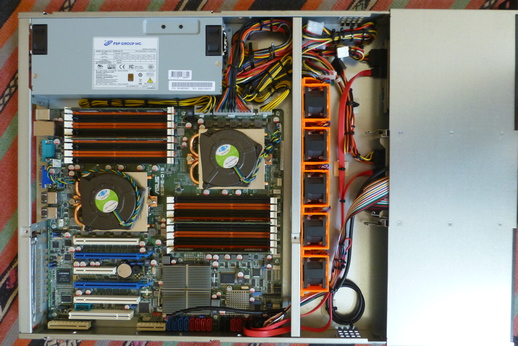
\includegraphics[width=\paperwidth]{images/libreboot-server}};
  \end{tikzpicture}

  \begin{tikzpicture}[overlay]
    \node<2>[rounded corners=4, text centered,
          fill=guixorange1, text width=8cm,
          inner sep=5mm, opacity=.75, text opacity=1,
          drop shadow={opacity=0.5}] at (current page.center) {
            \textbf{\Large{Libreboot inside! No ME™!}}
          };
  \end{tikzpicture}

  %% \begin{tikzpicture}[overlay]
  %%   \node<3>[rounded corners=4, text centered,
  %%         fill=guixorange1, text width=8cm, rotate=10,
  %%         inner sep=5mm, opacity=.75, text opacity=1, anchor=north east,
  %%         drop shadow={opacity=0.5}] at (current page.center) {
  %%           \Large{chewing new dog food soon...}
  %%         };
  %% \end{tikzpicture}
\end{frame}

\setbeamercolor{normal text}{bg=guixblue2}
\begin{frame}[plain]
  \Huge{\textbf{What's left before 1.0?}}
\end{frame}
\setbeamercolor{normal text}{fg=white,bg=black}

\begin{frame}[plain]{getting to 1.0}
  \Large{
    \begin{itemize}
    \item \texttt{guix pull} \& authenticated checkouts
    \item performance \& usability improvements
    \item{\highlight{GuixSD}
      \begin{itemize}
      \item encrypted root file system
      \item LVM support
      \item more system services
      \item fix bugs and glitches!
    \end{itemize}}
    \item self-hosted infra: \texttt{guix publish} and Cuirass
    \end{itemize}
  }
\end{frame}

\begin{frame}[plain]

  \vspace{0.7cm}
  \Large{
    \begin{itemize}
    \item \textbf{install the distribution}
    \item \textbf{use it}, report bugs, add packages
    \item help with the \textbf{infrastructure} + admin
    \item \textbf{donate} hardware/money
    \item share your \textbf{ideas}!
    \end{itemize}
  }

  \begin{textblock}{5}(7,8)
    \tikz
    \node[overlay, rounded corners=4, text centered,
          minimum size=10mm, fill=guixorange1, text width=5cm,
          inner sep=3mm, rotate=-7, opacity=.75, text opacity=1,
          drop shadow={opacity=0.5}] at (3, 3) {
            \textbf{your help needed!}
          };
  \end{textblock}
\end{frame}

%%%%%%%%%%%%%%%%%%%%%%%%%%%%%%%%%%%%%%%%%%%%%%%%%%%%%%%%%%%%%%%%%%%%%%%%%%%%%%
\begin{frame}[plain]

\vfill{
  \vspace{2.5cm}
  \center{
\includegraphics[width=0.3\textwidth]{images/GuixSD}}\\[1.0cm]
  \texttt{ludo@gnu.org}\hfill{\alert{\url{http://gnu.org/software/guix/}}}
}

\end{frame}

\begin{frame}{}

  \begin{textblock}{12}(2, 8)
    \tiny{
      Copyright \copyright{} 2010, 2012--2016 Ludovic Courtès \texttt{ludo@gnu.org}.\\[3.0mm]
      GNU GuixSD logo, CC-BY-SA 4.0, \url{http://gnu.org/s/guix/graphics}

      Copyright of other images included in this document is held by
      their respective owners.
      \\[3.0mm]
      This work is licensed under the \alert{Creative Commons
        Attribution-Share Alike 3.0} License.  To view a copy of this
      license, visit
      \url{http://creativecommons.org/licenses/by-sa/3.0/} or send a
      letter to Creative Commons, 171 Second Street, Suite 300, San
      Francisco, California, 94105, USA.
      \\[2.0mm]
      At your option, you may instead copy, distribute and/or modify
      this document under the terms of the \alert{GNU Free Documentation
        License, Version 1.3 or any later version} published by the Free
      Software Foundation; with no Invariant Sections, no Front-Cover
      Texts, and no Back-Cover Texts.  A copy of the license is
      available at \url{http://www.gnu.org/licenses/gfdl.html}.
      \\[2.0mm]
      % Give a link to the 'Transparent Copy', as per Section 3 of the GFDL.
      The source of this document is available from
      \url{http://git.sv.gnu.org/cgit/guix/maintenance.git}.
    }
  \end{textblock}
\end{frame}

\end{document}

% Local Variables:
% coding: utf-8
% comment-start: "%"
% comment-end: ""
% ispell-local-dictionary: "american"
% compile-command: "rubber --pdf talk.tex"
% End:

%%  LocalWords:  Reproducibility
